\documentclass[11pt]{amsbook}
\usepackage[utf8]{inputenc}
\usepackage[T1]{fontenc}
\usepackage{amsmath}
\usepackage{amsfonts}
\usepackage{amssymb}
\usepackage{amsthm}
\usepackage[version=4]{mhchem}
\usepackage{stmaryrd}
\usepackage{bbold}
\usepackage{graphicx}
\usepackage[export]{adjustbox}
\theoremstyle{plain}% default
\newtheorem{thm}{Theorem}[chapter]
\newtheorem{lem}[thm]{Lemma}
\newtheorem{prop}[thm]{Proposition}

\theoremstyle{definition}
\newtheorem{defn}{Definition}[section]
\newtheorem{exmp}{Example}[section]
\newtheorem{xca}[exmp]{Exercise}

\theoremstyle{remark}
\newtheorem*{rem}{Remark}
\newtheorem*{note}{Note}
\newtheorem{case}{Case}


\title{Notes on Lecture Series in Probability and Stochastic Processes }
\author{F. Wu}
\date{}

\def\Perp{\perp\!\!\!\perp}

\begin{document}
\maketitle
\tableofcontents
\part{Probability I}
\chapter{Measure theory}{Complements of Measure Theory and Topology}
\chapter{Random elements}{Randomness and Independence}
\chapter{Convergence}{Convergence Concepts, Laws of Large Numbers and Convergence of Series}
As usual and throughout this chapter, $(\Omega, \mathcal{F}, \mathbb{P})$ is our underlying probability space.
\begin{defn}
    A sequence of random variables $\left(X_{n}\right)_{n \geq 1}$ is said to converge in probability to a random variable $X_{\infty}$ if for all $\epsilon>0$, 
    \[\lim _{n \rightarrow+\infty} \mathbb{P}\left(\omega \in \Omega:\left|X_{n}(\omega)-X_{\infty}(\omega)\right| \geq \epsilon\right)=0.\]
\end{defn}

Above, the limiting random variable $X_{\infty}$ is almost surely unique since if two such limits $X_{\infty}$ and $Y_{\infty}$ do exist, then for any $\epsilon>0$,
$\mathbb{P}\left(\left|X_{\infty}-Y_{\infty}\right| \geq \epsilon\right)=0$, since $\left\{\left|X_{\infty}-Y_{\infty}\right| \geq \epsilon\right\} \subset$ $\left\{\left|X_{n}-X_{\infty}\right| \geq \epsilon / 2\right\} \cup\left\{\left|X_{n}-Y_{\infty}\right| \geq \epsilon / 2\right\}$. From which it follows that almost surely $X_{\infty}=Y_{\infty}$. Convergence in probability is then denoted by $X_{n} \xrightarrow{\mathbb{P}} X_{\infty}$.
This is the same as convergence point-wise almost everywhere in analysis.

\begin{defn}
    A sequence of random variables $\left(X_{n}\right)_{n>1}$ is said to converge almost surely (a.s.) to a random variable $X_{\infty}$ if there exists a null set $N \in \mathcal{F}$, such that for every $\omega \in N^{c}$, $\lim _{n \rightarrow+\infty}\left|X_{n}(\omega)-X_{\infty}(\omega)\right|=0$.
\end{defn}

Almost sure convergence is then denoted by $X_{n} \xrightarrow{\text { a.s. }} X_{\infty}$, and one also says that convergence holds with probability one. Clearly $X_{\infty}$ is also almost surely unique. This is the same as convergence in measure in analysis.

The next result precisely delineates almost sure convergence from convergence in probability.

\begin{prop} $X_{n} \xrightarrow{\text { a.s. }} X_{\infty}$ if and only if 
\begin{enumerate}
\item[(i)] for all $\epsilon>0, \lim _{n \rightarrow \infty} \mathbb{P}\left(\bigcup_{k=n}^{\infty}\left\{\left|X_{k}-X_{\infty}\right| \geq \epsilon\right\}\right)=0$,
\item[(ii)] $\mathbb{P}\left(\limsup _{n \rightarrow \infty}\left\{\left|X_{n}-X_{\infty}\right| \geq \epsilon\right\}\right)=0$,
\item[(iii)] for all $\epsilon>0$, $\varliminf_{n \rightarrow \infty} \mathbb{P}\left(\sup _{k \geq n}\left|X_{k}-X_{\infty}\right| \geq \epsilon\right)=0$.
\end{enumerate}
\end{prop}

\begin{proof}
Only (i) is proved since the proof of (ii) and (iii) is similar. For every $\epsilon>0$, let $A_{n}(\epsilon)=\left\{\left|X_{n}-X_{\infty}\right| \geq \epsilon\right\}, n \geq 1$. Let $D=\left\{\omega: X_{n}(\omega) \nrightarrow X_{\infty}(\omega)\right.$ as $\left.n \rightarrow+\infty\right\}$. Clearly, $D=\left\{\omega: \lim \sup _{n \rightarrow+\infty}\left|X_{n}(\omega)-X_{\infty}(\omega)\right|>0\right\}$, and so the set of divergence is also given by $D=\bigcup_{\epsilon>0} \limsup _{n \rightarrow \infty} A_{n}(\epsilon)$ which is clearly equal to $\bigcup_{k=1}^{\infty} \limsup _{n \rightarrow \infty} A_{n}(1 / k)$. Next, since $\underset{n \rightarrow \infty}{\limsup } A_{n}(1 / k) \subset D$, and since $\mathbb{P}(D) \leq \sum_{k=1}^{\infty} \mathbb{P}\left(\underset{n \rightarrow \infty}{\limsup } A_{n}(1 / k)\right), \mathbb{P}(D)=0$ if and only if $\mathbb{P}\left(\underset{n \rightarrow \infty}{\limsup } A_{n}(1 / k)\right)=0$, for all $k$. But $\bigcup_{m=n}^{\infty} A_{n}(\epsilon) \downarrow \limsup A_{n}(\epsilon)$, hence $\mathbb{P}\left(\limsup _{n \rightarrow \infty} A_{n}(\epsilon)\right)=$ $\lim _{n \rightarrow \infty} \mathbb{P}\left(\bigcup_{m=n}^{\infty} A_{n}(\epsilon)\right)$.
\end{proof} 

Remark 3.4. (i) Above the result is non vacuous since $\left\{\limsup _{n \rightarrow \infty}\left|X_{n}-X_{\infty}\right| \geq \epsilon\right\} \subset$ $\lim \sup _{n \rightarrow \infty}\left\{\left|X_{n}-X_{\infty}\right| \geq \epsilon\right\}$\\

(ii) As a direct consequence of the above almost sure convergence implies convergence in probability. In fact, this implication is clear since for each $\epsilon>0$, the sequence $\left(\mathbf{1}_{\left|X_{n}-X_{\infty}\right| \geq \epsilon}\right)_{n \geq 1}$ converges almost surely to zero and is dominated by 1.

The converse is not true. Indeed, let $\left(X_{n}\right)_{n \geq 1}$ be a sequence of Bernoulli random variables each with parameter $p_{n}$. Then,

$$
\mathbb{P}\left(\left|X_{n}\right| \geq \epsilon\right)= \begin{cases}0 & \text { if } \epsilon>1 \\ p_{n} & \text { if } 0<\epsilon \leq 1\end{cases}
$$

Therefore, for all $\epsilon>0$,

$$
\lim _{n \rightarrow+\infty} \mathbb{P}\left(\left|X_{n}\right| \geq \epsilon\right) \leq \lim _{n \rightarrow+\infty} p_{n}
$$

and convergence in probability to zero is equivalent to $\lim _{n \rightarrow+\infty} p_{n}=0$. On the other hand, by the previous proposition, a.s. convergence is equivalent to $\mathbb{P}\left(\left\{\left|X_{n}-X_{\infty}\right| \geq \epsilon\right\}\right.$ i.o. $)=0$, which when the random variables $X_{n}$ are independent is in turn equivalent, thanks to the Borel-Cantelli Lemma, to $\sum_{n=1}^{\infty} \mathbb{P}\left(\left|X_{n}-X_{\infty}\right| \geq \epsilon\right)<+\infty$. So a.s. convergence to zero of the sequence $\left(X_{n}\right)_{n \geq 1}$ of independent Bernoulli random variables each with parameter $p_{n}$ is equivalent to $\sum_{n=1}^{\infty} p_{n}<+\infty$. Moreover, by Kolmogorov zero-one law,

$$
\begin{aligned}
& \mathbb{P}\left(\sum X_{n}<+\infty\right)=1 \quad \text { if } \sum p_{n}<+\infty \\
& \mathbb{P}\left(\sum X_{n}<+\infty\right)=0 \quad \text { if } \sum p_{n}=+\infty
\end{aligned}
$$

Here is a generic summary of what was just described.\\
Corollary 3.5. Let $\left(X_{n}\right)_{n \geq 1}$ be completely convergent towards $X_{\infty}$, i.e., let $\sum_{n=1}^{\infty} \mathbb{P}\left(\mid X_{n}-\right.$ $\left.X_{\infty} \mid \geq \epsilon\right)<+\infty$, for all $\epsilon>0$. Then $X_{n} \xrightarrow{\text { a.s. }} X_{\infty}$. The converse is true if the $X_{n}$ are independent.

Proof. Let $\epsilon>0$. Then, $\mathbb{P}\left(\bigcup_{m=n}^{\infty}\left\{\left|X_{m}-X_{\infty}\right| \geq \epsilon\right\}\right) \leq \sum_{m=n}^{\infty} \mathbb{P}\left(\left|X_{m}-X_{\infty}\right| \geq \epsilon\right)$. But, $\sum_{n=1}^{\infty} \mathbb{P}\left(\left|X_{n}-X_{\infty}\right| \geq \epsilon\right)<+\infty$, and so the remainder of the series converges to zero which by the previous proposition ensures that $X_{n} \xrightarrow{\text { a.s. }} X_{\infty}$. For the converse, the events $\left\{\left|X_{n}-X_{\infty}\right| \geq \epsilon\right\}$ are independent events and so by the Borel-Cantelli Lemma,

$$
\mathbb{P}\left(\limsup _{n \rightarrow \infty}\left\{\left|X_{n}-X_{\infty}\right| \geq \epsilon\right\}\right)=0,
$$

which implies that $\sum_{n=1}^{\infty} \mathbb{P}\left(\left|X_{n}-X_{\infty}\right| \geq \epsilon\right)<+\infty$.\\
Somehow, the above result quantify how fast convergence in probability must be in order to become almost sure convergence. In the very definition of complete convergence, and by the Borel-cantelli lemma, one could replace $\epsilon>0$ by any sequence $\left(\epsilon_{n}\right)_{n \geq 1} \downarrow 0$. When independence is not assumed, then the converse result is no longer true as the sequence $X_{n}=\mathbf{1}_{(0,1 / n]}$ shows. Indeed, $\limsup X_{n}=\mathbf{1}_{\emptyset}=0$, but whenever $\mathbb{P}$ is the uniform measure on $(0,1], \sum \mathbb{P}\left(\left|X_{n}\right| \geq \epsilon\right)=\sum 1 / n=+\infty$, for any $0<\epsilon<1$.

Amid the lack of a converse implication of convergence in probability to a.s. convergence, there is nevertheless:\\

\includegraphics[max width=\textwidth, center]{2024_11_17_7987aa6f5f165d92ff66g-03}

Proposition 3.6. If $X_{n} \xrightarrow{\mathrm{P}} X_{\infty}$, then there exists a subsequence $\left(X_{n_{k}}\right)$ such that $X_{n_{k}} \xrightarrow{\text { as }} X_{\infty}$.\\
Proof. For all $k>0, \lim _{n \rightarrow+\infty} \mathbb{P}\left(\left|X_{n}-X_{\infty}\right| \geq 1 / 2^{k}\right)=0$. Hence for each $k$, there exists $n_{k}$ such that $\mathbb{P}\left(\left|X_{n_{k}}-X_{\infty}\right| \geq 1 / 2^{k}\right) \leq 1 / 2^{k}$. But $\sum \mathbb{P}\left(\left|X_{n_{k}}-X_{\infty}\right| \geq 1 / 2^{k}\right) \leq \sum_{k} 1 / 2^{k}<$ $+\infty$. Hence by the Borel-Cantelli lemma,

$$
\mathbb{P}\left(\underset{k}{\left.\limsup \left\{\left|X_{n_{k}}-X_{\infty}\right| \geq 1 / 2^{k}\right\}\right)}=0\right.
$$

In other words, if $N=\limsup \left\{\left|X_{n_{k}}-X_{\infty}\right| \geq 1 / 2^{k}\right\}$, we have $\mathbb{P}\left(N^{c}\right)=1$. Thus, for each $\omega \in N^{c}$, there exists an integer $\ell=\ell(\omega)$ (which also depends on $k$ ) such that

$$
\left|X_{n_{\star}}(\omega)-X_{\infty}(\omega)\right| \leq \frac{1}{2^{k}}, \quad \text { for all } k \geq \ell(\omega)
$$

Thus, $X_{n_{k}}(\omega) \rightarrow X_{\infty}(\omega)$. In other words, $\mathbb{P}(N)=0$ if and only if $\mathbb{P}(\omega \in$ infinitely many $\left.\left\{\left|X_{n_{k}}-X_{\infty}\right| \geq 1 / 2^{k}\right\}\right)=0$.

Definition 3.7. The sequence $\left(X_{n}\right)_{n \geq 1}$ is said to be a.s. a Cauchy sequence if there exists a null set $N \in \mathcal{F}$, such that for every $\omega \in N^{c}, \lim _{n, m \rightarrow \infty}\left|X_{n}(\omega)-X_{m}(\omega)\right|=0$.

It is well known that $\mathbb{R}$ is complete, and so $X_{n} \rightarrow X_{\infty}$ a.s. if and only if $\left(X_{n}\right)_{n \geq 1}$ is a Cauchy sequence for a.s. convergence. Here is a statement which is the pendant of Proposition 3.3\\
$\left(X_{n}\right)_{n \geq 1}$ is Cauchy for almost sure convergence if and only if for all $\epsilon>0$,

$$
\lim _{n \rightarrow \infty} \mathbb{P}\left(\bigcup_{m=1}^{\infty}\left\{\left|X_{m+n}-X_{n}\right| \geq \epsilon\right\}\right)=0
$$

if and only if for all $\epsilon>0, \lim _{n \rightarrow \infty} \mathbb{P}\left(\sup _{k \geq 1}\left|X_{n+k}-X_{n}\right| \geq \epsilon\right)=0$.\\
In complete similarity to the notion of almost sure Cauchy sequence, we have the notion of Cauchy sequence in probability, more precisely $\left(X_{n}\right)_{n \geq 1}$ is a Cauchy sequence for convergence in probability if $\mathbb{P}\left(\omega \in \Omega:\left|X_{n}(\omega)-X_{m}(\omega)\right| \geq \epsilon\right) \xrightarrow[n, m \rightarrow \infty]{\longrightarrow} 0$. In fact,\\
Proposition 3.8. $X_{n} \xrightarrow{\mathrm{P}} X_{\infty}$ if and only if $\left(X_{n}\right)_{n \geq 1}$ is a Cauchy sequence for convergence in probability.

Proof. For the direct implication,

$$
\left|X_{n}-X_{m}\right| \leq\left|X_{n}-X_{\infty}\right|+\left|X_{m}-X_{\infty}\right| .
$$

Hence,

$$
\left\{\left|X_{n}-X_{m}\right| \geq \epsilon\right\} \subset\left\{\left|X_{n}-X_{\infty}\right| \geq \frac{\epsilon}{2}\right\} \cup\left\{\left|X_{n}-X_{\infty}\right| \geq \frac{\epsilon}{2}\right\}
$$

and thus

$$
\mathbb{P}\left(\left|X_{n}-X_{m}\right| \geq \epsilon\right) \leq \mathbb{P}\left(\left|X_{n}-X_{\infty}\right| \geq \frac{\epsilon}{2}\right)+\mathbb{P}\left(\left|X_{m}-X_{\infty}\right| \geq \frac{\epsilon}{2}\right),
$$

and both last terms converge to zero as $n$ goes to infinity. For the converse, if $\left(X_{n}\right)_{n \geq 1}$ is Cauchy in probability, hence there exists a random variable $X_{\infty}$ such that $X_{n_{k}} \rightarrow X_{\infty}$ a.s. (and thus $X_{n_{\star}} \xrightarrow{\mathrm{p}} X_{\infty}$ ).

$$
\mathbb{P}\left(\left|X_{n}-X_{\infty}\right| \geq \epsilon\right) \leq \mathbb{P}\left(\left|X_{n}-X_{n_{k}}\right| \geq \frac{\epsilon}{2}\right)+\mathbb{P}\left(\left|X_{n_{k}}-X_{\infty}\right| \geq \frac{\epsilon}{2}\right),
$$

and both terms converge to zero.\\
Before continuing studying convergence concepts, let us present three important inequalities involving tails.

The simplest and better known is the Bienaymé-Chebyshev-Markov Inequality which asserts that if $X \geq 0$ is a non negative random variable and if $h:[0,+\infty[: \rightarrow] 0,+\infty[$, is non decreasing and such that $\mathbb{E} h(X)<+\infty$, then for all $\epsilon>0$,

$$
\mathbb{P}(X \geq \epsilon) \leq \frac{\mathbb{E} h(X)}{h(\epsilon)}
$$

Proof.

$$
\mathbb{E} h(X)=\int_{\Omega} h(X) d \mathbb{P} \geq \int_{X \geq \epsilon} h(X) d \mathbb{P} \geq h(\epsilon) \mathbb{P}(X \geq \epsilon)
$$

Some particular cases worth noting: $h(x)=x^{p}$, another consequence of the above which is worth nothing is that whenever $X$ is a random variable such that $\mathbb{E}|X|^{p}<+\infty$, for some $p>0$, then

$$
\mathbb{P}(|X-\mathbb{E} X| \geq \epsilon) \leq \frac{\mathbb{E}|X-\mathbb{E} X|^{p}}{\epsilon^{p}}
$$

Second, let $X$ and $h$ be as above, assume moreover that $h(X)$ is essentially bounded and denote by $\|h(X)\|_{\infty}$ the corresponding supremum. Then for all $\epsilon>0$,

$$
\mathbb{P}(X \geq \epsilon) \geq \frac{\mathbb{E} h(X)-h(\epsilon)}{\|h(X)\|_{\infty}}
$$

Proof.

$$
\begin{aligned}
\mathbb{E} h(X) & =\int_{X \geq \epsilon} h(X) d \mathbb{P}+\int_{X<\epsilon} h(X) d \mathbb{P} \\
& \leq\|h(X)\|_{\infty} \int_{X \geq \epsilon} d \mathbb{P}+h(\epsilon) \int_{X<\epsilon} d \mathbb{P} \\
& \leq\|h(X)\|_{\infty} \mathbb{P}(X \geq \epsilon)+h(\epsilon) .
\end{aligned}
$$

Of course, this last inequality does present an interest only when $\epsilon$ is such that $\mathbb{E} h(X)>$ $h(\epsilon)$ it has however other virtues, one of which is to lead to our next proposition. But before:

The third inequality is the Paley-Zygmund one, a rare case where a lower bound can be provided: Let $X \geq 0$ be a nonnegative random variable with finite second moment, then for all $0<\lambda<1$,

$$
(1-\lambda)^{2} \frac{(\mathbb{E} X)^{2}}{\mathbb{E} X^{2}} \leq \mathbb{P}(X \geq \lambda \mathbb{E} X)
$$

Proof.

$$
\mathbb{E} X=\mathbb{E}\left(X 1_{X \gtrless \mathcal{E} X}\right)+\mathbb{E}\left(X 1_{X \leq X \mathbb{E} X}\right) \leq \mathbb{E} X 1_{X \gtrless \mathbb{E} X}+\lambda \mathbb{E} X,
$$

Therefore,

$$
(1-\lambda) \mathbb{E} X \leq \sqrt{\mathbb{E} X^{2}} \sqrt{\mathbb{P}(X \geq \lambda \mathbb{E} X)},
$$

$$
(1-\lambda)^{2} \frac{(\mathbb{E} X)^{2}}{\mathbb{E} X^{2}} \leq \mathbb{P}(X \geq \lambda \mathbb{E} X) .
$$

Add some exponential inequalities ?\\
To conclude this part we show as an application of the Paley-Zygmund inequality another proof of the direct part of the Borel-Cantelli Lemma.\\
(Borel $0-1$ Law) If $\sum_{n} \mathbb{P}\left(A_{n}\right)<+\infty$, then $\mathbb{P}\left(A_{n}\right.$ i.o. $)=0$.\\
Proposition 3.9. Let $p>0$. Then, $X_{n} \xrightarrow{\mathrm{P}} 0$ if and only if $\mathbb{E}\left(\frac{\left|X_{n}\right|^{p}}{1+\left|X_{n}\right|^{p}}\right) \rightarrow 0$.\\
Proof. Combining the first and second inequalities above gives:

$$
\mathbb{E}\left(\frac{\left|X_{n}\right|^{p}}{1+\left|X_{n}\right|^{p}}\right)-\frac{\epsilon^{p}}{1+\epsilon^{p}} \leq \mathbb{P}\left(\left|X_{n}\right| \geq \epsilon\right) \leq \frac{1+\epsilon^{p}}{\epsilon^{p}} \mathbb{E}\left(\frac{\left|X_{n}\right|^{p}}{1+\left|X_{n}\right|^{p}}\right) .
$$

Definition 3.10. Let $\left(X_{n}\right)_{n \geq 1}$ be a sequence of random variables such that $\mathbb{E}\left|X_{n}\right|^{p}<+\infty$, $0<p<+\infty$. Then, $\left(X_{n}\right)_{n \geq 1}$ is said to converge in the $p$ th mean to a random variable $X_{\infty}$ such that $\mathbb{E}\left|X_{\infty}\right|^{p}<+\infty$ if $\mathbb{E}\left|X_{n}-X_{\infty}\right|^{p} \underset{n \rightarrow \infty}{\longrightarrow} 0$.

We write $X_{n} \xrightarrow{L P} X$, and again the limiting random variable if it exists is (a.s.) unique. Definition 3.11. A sequence of random variables $\left(X_{n}\right)_{n \geq 1}$ is said to be Cauchy in the $p$ th mean if $\mathbb{E}\left|X_{n}-X_{m}\right|^{p} \underset{n, m}{\longrightarrow} 0$.

As well known, for pth mean convergence, there is equivalence between the notion of convergent and Cauchy sequence. As also well known:\\
Proposition 3.12. If $X_{n} \xrightarrow{L^{P}} X_{\infty}$, then $X_{n} \xrightarrow{\mathrm{P}} X_{\infty}$.\\
Proof. $\mathbb{P}\left(\left|X_{n}-X_{\infty}\right| \geq \epsilon\right) \leq \mathbb{E}\left|X_{n}-X_{\infty}\right|^{p} / \epsilon^{p}$.\\
In general, convergence in probability does not imply convergence in $L^{p}$. Indeed, take $(\Omega, \mathcal{F}, \mathbb{P})=((0,1], \mathcal{B}((0,1])$, Leb. $)$ and let $X_{n}=n^{1 / p} 1_{(0,1 / n \mid}$. Then, $\mathbb{E}\left|X_{n}\right|^{p}=1$, but $\mathbb{P}\left(\left|X_{n}\right| \geq\right.$ $\epsilon)=1 / n \rightarrow 0$ as $n \rightarrow+\infty$, moreover with probability one, $\limsup _{n \rightarrow \infty} X_{n}=0$ and so almost sure convergence does not imply pth mean convergence. Note also that if $\left(X_{n}\right)_{n \geq 1}$ is a sequence of Bernoulli random variables, each with parameter $p_{n}$, then $X_{n} \xrightarrow{L^{p}} 0$ is equivalent to $\lim _{n \rightarrow+\infty} p_{n}=0$ which is equivalent to $X_{n} \xrightarrow{\mathrm{P}} 0$. Hence convergence in the $p$ th mean does not imply almost sure convergence either.

Recall that $D^{p}:=L^{P}(\Omega, \mathcal{F}, \mathbb{P})=\left\{X: \Omega \rightarrow \mathbb{R}: \mathbb{E}|X|^{P}<+\infty\right\}$ is a (real) Bensch space with norm given by $\|X\|_{p}=\left(\mathbb{E}|X|^{P}\right)^{1 / p}, 1 \leq p<+\infty$, and so is $L^{\infty}:=L^{\infty}(\Omega, \mathcal{F}, \mathbb{P})=\{X$ : $\left.\operatorname{Nin}_{\Omega \rightarrow \mathbb{R}}: \operatorname{esssup}|X|<+\infty\right\}$ with $\|X\|_{\infty}:=\operatorname{ess} \sup |X|=\inf \{M>0$ s.t. $|X| \leq M$ a.s. $\}$. For $p=2, L^{2}$ is a (real) Hilbert space. For $0<p<1,(\mathbb{E}|\cdot| P)^{1 / p}$ does not satisfy the triangle inequality (only up to a multiplicative constant depending on $p$ ), and thus it is a quasi-norm and $D P, O<p<1$ is a quasi-Banach space. Still for $0<p<1$, $L^{P}$ is a metric space with distance given by $E|X=Y| P$.

Now, $L^{0}:=L^{0}(\Omega, F, \mathbb{P})=\{X: \Omega \rightarrow \mathbb{R}\}$, is a (real) vector space, and the untural copology on $L^{0}$ is the one induced by convergence in probability.\\
Proposition 3.13. For $X, Y \in L^{0}(\Omega, \mathcal{F}, \mathbb{P})$, let $d(X, Y)=\mathbb{E}\left(\frac{|X-Y|}{1+|X-Y|}\right)$. Then $d$ is a metric which is equivalent to convergence in probability.\\
Proof. It is clear that $d(X, Y)=0$ if and only if with probability one $X=Y$. next, it is also clear that $d(X, Y)=d(Y, X)$, and we just need to prove the triangle inequality: $d(X, Z) \leq d(X, Y)+d(Y, Z)$. To do so, it is enough to show that

$$
\frac{|x+y|}{1+|x+y|} \leq \frac{|x|}{1+|x|}+\frac{|y|}{1+|y|}, \quad \forall x, y \in \mathbb{R}
$$

because $X-Z=(X-Y)+(Y-Z)$. Assume that $|y| \leq|x|$ (which is without loss of generality by symmetry)

$$
\begin{aligned}
\frac{|x+y|}{1+|x+y|}-\frac{|x|}{1+|x|} & =\frac{(1+|x|)(|x+y|)-|x|(1+|x+y|)}{(1+|x|)(1+|x+y|)} \\
& =\frac{|x+y|-|x|}{(1+|x+y|)(1+|x|)} \\
& \leq \frac{\|x+y|-| x\|}{1+|x|} \\
& \leq \frac{|y|}{1+|y|} .
\end{aligned}
$$

Hence $d$ is a metric, and the equivalence to convergence in probability is a consequence of Proposition 3.9.

Rewording the above result differently, we say that $d$ metrizes convergence in probability, i.e., $X_{n} \xrightarrow{\mathrm{P}} X \Leftrightarrow d\left(X_{n}, X\right) \rightarrow 0$. In fact, $\left(L^{0}, d\right)$ is a complete metric space. There are many ways to metrize convergence in probability. Another popular one $d(X, Y)=\mathbb{E} \arctan |X-Y|$, a third way is via $d(X, Y)=\mathbb{E} \min (1,|X-Y|)$.

Let us present some further results on convergence in probability. First, a small lemma which is harder to state than to prove.\\
Lemma 3.14. Let $\left(x_{n}\right)_{n \geq 1}$ be a sequence of elements of a metric space $(M, d)$. The sequence $\left(x_{n}\right)_{n \geq 1}$ converges to $x_{\infty}$ in $(M, d)$ if and only if from every subsequence $\left(x_{n(m)}\right)$ one can extract a further subsequence $\left(x_{n(m(k))}\right)$ converging to $x_{\infty}$.\\
Proof. The direct implication is clear. For the converse, if not, then there exists $\epsilon>0$, such that for any $n \geq 1$, there exists $m \geq n$ with $d\left(x_{m}, x_{\infty}\right)>\epsilon$. In other words, there exists $\epsilon>0$ and a subsequence $m(n)$ such that $d\left(x_{m(n)}, x_{\infty}\right)>\epsilon$. But, $d\left(x_{m(n(k))}, x_{\infty}\right) \rightarrow 0$, for a subsequence $m(n(k))$ of $m(n)$, leading to a contradiction.\\
proposition 3.15. $X_{n} \rightarrow X_{\infty}$ in probability if and only if for every subsequence ( $\left.X_{n(m)}\right)$. chere is a further subsequence $\left(X_{n(m / k))}\right)$ such that $X_{n(m(k))}$ converges to $X_{\infty 0}$, in probability proof. A first proof is to combined the previous lemms with the previous proposition. Direct arguments will go as follows: If $X_{n} \xrightarrow{\mathrm{P}} X_{\infty}$, then $X_{n(m)} \rightarrow X_{\infty}$ in probability and then there exists a subsequence such that $X_{n(m / k))} \xrightarrow{\mathrm{as}} X_{\infty}$. Conversely use the previous lemma with $x_{n}=\mathbb{P}\left(\left|X_{n}-X_{\infty}\right| \geq c\right)$. An alternate proof of the converse is as follows. If not, i.e., if $X_{n} \nrightarrow X_{\infty}$ in probability. Then for each $\epsilon>0$ there exists a subsequence $n(m)$ such that $\mathbb{P}\left(\left|X_{n(m)}-X_{\infty}\right|>\varepsilon\right) \nrightarrow 0$. But $X_{\mathrm{n}(m(k))} \xrightarrow{\mathbb{P}} X_{\infty}$.

At this point, one might wonder whether or not it is possible to metrize almost sure convergence. Indeed, let us assume that this is the case (or even more generally that almost sure convergence can be topologized). Then by the above lemma, $\left(X_{n}\right)_{n \geq 1}$ converges almost surely to $X_{\infty}$ if and only if one can extract from any subsequence ( $X_{n(m)}$ ) a further subsequence $\left(X_{n(m(k))}\right)$ converging to $X_{\infty}$ almost surely. Now, let $\left(X_{n}\right)_{n \geq 1}$ be a sequence of Bernoulli random variables converging to $X_{\infty}$ in probability but not almost surely. Then, any subsequence of $\left(X_{n}\right)_{n \geq 1}$ also converges to $X_{\infty}$ in probability and therefore from this subsequence one can extract a further subsequence converging almost surely to $X_{\infty}$. However, $\left(X_{n}\right)_{n \geq 1}$ does not converge almost surely to $X_{\infty}$ and we have reached a contradiction.

The above proposition is rather useful and shows, for example, that dominated convergence (or Fatou's lemma) hold under a convergence in probability assumption.\\
Proposition 3.16. Let $\left(X_{n}\right)_{n \geq 1}$ be a sequence of random variables converging in probability to $X_{\infty}$ and such that for all $n \geq 1,\left|X_{n}\right| \leq Y \in L^{1}$. Then, $\lim _{n \rightarrow+\infty} \mathbb{E}\left|X_{n}-X_{\infty}\right|=0$.\\
Proof. Let $\left(X_{n(m)}\right)$ be a subsequence of $\left(X_{n}\right)$. As $\left(X_{n(m)}\right)$ converges to $X_{\infty}$ in probability, one can extract a sub-subsequence $\left(X_{n(m(k)))}\right)$ converging a.s. to $X_{\infty}$. But, $\left|X_{n(m(k))}\right| \leq Y \in$ $L^{1}$, and so by the dominated convergence theorem, $\lim _{n(m(k)) \rightarrow+\infty} \mathbb{E}\left|X_{n(m(k))}-X_{\infty}\right|=0$. Therefore by the previous proposition, $\lim _{n \rightarrow+\infty} \mathbb{E}\left|X_{n}-X_{\infty}\right|=0$.

Here is another example of the usefulness of the previous Proposition 3.14.\\
Corollary 3.17. Let $f$ be continuous and let $X_{n} \xrightarrow{\mathrm{P}} X_{\infty}$, then $f\left(X_{n}\right) \xrightarrow{\mathrm{P}} f\left(X_{\infty}\right)$. If in addition $f$ is bounded, then $\mathbb{E} f\left(X_{n}\right) \rightarrow \mathbb{E} f\left(X_{\infty}\right)$.\\
Proof. If $X_{n(m)}$ is a subsequence of $X_{n}$ then there is $X_{n(m(k))}$ such that $X_{n(m(k))} \xrightarrow{\text { a.s. }} X_{\infty}$. But since $f$ is continuous, $f\left(X_{n(m(k))}\right) \xrightarrow{\text { a.e. }} f\left(X_{\infty}\right)$. Hence $f\left(X_{n}\right) \rightarrow f\left(X_{\infty}\right)$ in probability: Now if $f$ is bounded, then by bounded convergence we have $\mathbb{E} f\left(X_{n(m(k))}\right) \rightarrow \mathbb{E} f\left(X_{\infty}\right)$ and apply Lemma 3.14 to $x_{n}=\mathbb{E} f\left(X_{n}\right)$.

Motivated by the previous result, let us introduce next a type of convergence which will prove fundamental in the sequel and which, by the previous proposition, is implied by (and thus weaker than) convergence in probability (but not conversely).\\
Definition 3.18. A sequence $\left(X_{n}\right)_{n \geq 1}$ is said to converge in distribution (or in law or weakly) to a random variable $X_{\infty}$, if for any real-valued bounded continuous function $f$ defined on $\mathbb{R}, \lim _{n \rightarrow+\infty} \mathbb{E} f\left(X_{n}\right)=\mathbb{E} f\left(X_{\infty}\right)$.

This last type of convergence is often written as $X_{n} \xrightarrow{d} X_{\infty}$, or $X_{n} \xrightarrow{\mathcal{L}} X_{\infty}$, or $X_{n} \xrightarrow{w} X_{\infty}$, or $X_{n} \Longrightarrow X_{\infty}$.

Here is an example showing that convergence in distribution does not imply convergence in probability, Let $X$ and $Y$ be two iid Bernoulli random variables with $\mathbb{P}(X=0)=\mathbb{P}(X=$ 1) $=1 / 2$, and let $X_{n}=Y$, for all $n \geq 1$. (Assume also that all thes ${ }^{P}$. defined on the same probability space.) Then $X_{n} \Rightarrow X$ in law, but $X_{n} \leftrightarrows$. Indeed, for any $0<\epsilon<1$,

$$
\begin{aligned}
\mathbb{P}\left(\left|X_{n}-X\right| \geq \epsilon\right) & =\mathbb{P}(|Y-X| \geq \epsilon) \\
& =\mathbb{P}(Y=1, X=0)+\mathbb{P}(Y=0, X=1) \\
& =\frac{1}{2} .
\end{aligned}
$$

There are nevertheless partial converse (the converging together lemma) which we will explore later.

Let us now delineate convergence in probability from convergence in the $p$ th mean.\\
Definition 3.19. A collection of random variables, $\left(X_{t}\right)_{t \in T}$ is called uniformly integrable (or equi-integrable) if

$$
\lim _{M \rightarrow+\infty} \sup _{t \in T} \int_{\left|X_{t}\right|>M}\left|X_{t}\right| d \mathbb{P}=0
$$

Let $\left(X_{n}\right)_{n \geq 1}$ be such that $\mathbb{P}\left(X_{n}=n\right)=1 / n^{2}$ and $\mathbb{P}\left(X_{n}=0\right)=1-1 / n^{2}$. Then $\left(X_{n}\right)_{n \geq 1}$ is uniformly integrable since $\int_{\left|X_{n}\right|>M}\left|X_{n}\right| d \mathbb{P}$ is either equal to 0 or $1 / n$ according to $n \leq \bar{M}$ or $n>M$. Thus, $\sup _{n} \int_{\left|X_{n}\right|>M}\left|X_{n}\right| d \mathbb{P} \leq 1 / M$. On the other hand, the sequence $\left(Y_{n}\right)_{n \geq 1}$ be such that $\mathbb{P}\left(Y_{n}=n\right)=1 / n$ and $\mathbb{P}\left(Y_{n}=0\right)=1-1 / n$ is not uniformly integrable as $\sup _{n} \int_{\left|X_{n}\right|>M}\left|X_{n}\right| d \mathbb{P}=1$.\\
Theorem 3.20. $\left(X_{t}\right)_{t \in T}$ is uniformly integrable if and only if the following two conditions are satisfied:\\
(i) $\mathbb{E}\left|X_{t}\right| \leq C$ (independent of $t \in T$ ).\\
(ii) $\forall \epsilon>0, \exists \delta=\delta(\epsilon)>0: \forall A \in \mathcal{F}$ with $\mathbb{P}(A)<\delta, \sup _{t \in T} \int_{A}\left|X_{t}\right| d \mathbb{P}<\epsilon$.

Proof. Clearly, uniform integrability implies (i). Next, let $A \in \mathcal{F}$ and let $B_{t}=\left\{\left|X_{t}\right|>M\right\}$.

$$
\begin{aligned}
\int_{A}\left|X_{t}\right| d \mathbb{P} & =\int_{A \cap B_{t}}\left|X_{t}\right| d \mathbb{P}+\int_{A \cap A_{t}^{c}}\left|X_{t}\right| d \mathbb{P} \\
& \leq \int_{A \cap B_{t}}\left|X_{t}\right| d \mathbb{P}+M \mathbb{P}\left(A \cap B_{t}^{c}\right) \\
& \leq \int_{\left|X_{t}\right|>M}\left|X_{t}\right| d \mathbb{P}+M \mathbb{P}(A)
\end{aligned}
$$

Now by uniform integrability, given $\epsilon>0$, there exists $M(\epsilon)$ such that $\sup _{t \in T} \int_{\left|X_{t}\right|>M}\left|X_{t}\right| d \mathbb{P} \leq$ $\epsilon / 2$. Next, taking $\delta=\epsilon / 2 M$, then clearly $M \mathbb{P}(A) \leq \epsilon / 2$, and the result follows.

For the converse implication, $\mathbb{P}\left(\left|X_{t}\right|>M\right) \leq \mathbb{E}\left|X_{t}\right| / M \leq C / M$. Hence, if $M>C / \delta$ then $\mathbb{P}\left(\left|X_{t}\right|>M\right)<\delta$, and so $\sup _{t \in T} \int_{\left|X_{t}\right|>M}\left|X_{t}\right| d \mathbb{P}<\epsilon$.

Uniform integrability is just what is needed to understand the difference between convergence in probability and convergence in the pth mean.

Theorem 3.21. Let $0<p<+\infty$, let $\left(X_{n}\right)_{n \geq 1}$ be a sequence of random variables such that $X_{n} \in L^{p}$, and $X_{n} \xrightarrow{\mathrm{P}} X_{\infty}$. The following are equivalent\\
(i) $\left(\left|X_{n}\right|^{p}\right)_{n \geq 1}$ is uniformly integrable.\\
(ii) $X_{n} \xrightarrow{L P} X_{\infty}$.\\
(iii) $\mathbb{E}\left|X_{n}\right|^{p} \rightarrow \mathbb{E}\left|X_{\infty}\right|^{p}$.

Proof. Assume that $\left(\left|X_{n}\right|^{p}\right)_{n \geq 1}$ is uniform il , with probability one. Then,\\
subsequence $\left(X_{n(m)}\right)$ such that $X_{n(m)} \rightarrow X_{\infty}$, with probability

$$
\int_{\Omega}\left|X_{\infty}\right|^{p} d \mathbb{P}=\int_{\Omega} \liminf \left|X_{n(m)}\right|^{p} d \mathbb{P} \leq \liminf \int_{\Omega}\left|X_{n(m)}\right|^{p} d \mathbb{P} \leq C \text {, }
$$

and so $X_{\infty} \in L^{p}$. But, $\left|X_{n}-X_{\infty}\right|^{p} \leq \max \left(1,2^{p-1}\right)\left(\left|X_{n}\right|^{p}+\left|X_{\infty}\right|^{p}\right.$, and so uniform integraability implies that $\left(\left|X_{n}-X_{\infty}\right|^{p}\right)_{n \geq 1}$ is also uniformly integrable. Next, for each $\epsilon>0$,

$$
\begin{aligned}
& \mathbb{E}\left|X_{n}-X_{\infty}\right|^{p} \\
& =\mathbb{E}\left|X_{n}-X_{\infty}\right|^{p} 1_{\left|X_{n}-X_{\infty}\right| \geq c}+\mathbb{E}\left|X_{n}-X_{\infty}\right|^{p} 1_{\mid X_{n}}-X_{\infty} \mid<\epsilon \\
& \\
& \\
& \leq \mathbb{E}\left|X_{n}-X_{\infty}\right|^{p} 1_{\left|X_{n}-X_{\infty}\right| \geq c}+\epsilon^{p}
\end{aligned}
$$

Since $\mathbb{P}\left(\left|X_{n}-X_{\infty}\right| \geq \epsilon\right) \underset{n \rightarrow+\infty}{\longrightarrow} 0$, it follows from (ii) of the previous theorem that

$$
\limsup _{n \rightarrow+\infty}^{+\infty} \mathbb{E}\left|X_{n}-X_{\infty}\right|^{p} 1_{\left|X_{n}-X_{\infty}\right| \geq \epsilon}=0 .
$$

Therefore, (i) implies (ii).\\
The implication (ii) $\Rightarrow$ (iii) follows from the triangle inequality when $p \geq 1$, while for $0<p<1$ it follows from the easy inequality

$$
\left|X_{n}\right|^{p}-\left|X_{n}-X_{\infty}\right|^{p} \leq\left|X_{\infty}\right|^{p} \leq\left|X_{n}\right|^{p}+\left|X_{n}-X_{\infty}\right|^{p} .
$$

Let us now tackle the last implication (iii) $\Rightarrow$ (i). $\left|X_{n}-X_{\infty}\right|^{p} \leq \max \left(1,2^{p-1}\right)\left(\left|X_{n}\right|^{p}+\right.$ $\left.\left|X_{\infty}\right|^{p}\right)$. Hence $0 \leq \max \left(1,2^{p-1}\right)\left(\left|X_{n}\right|^{p}+\left|X_{\infty}\right|^{p}\right)-\left|X_{n}-X_{\infty}\right|^{p}$. But $X_{n} \xrightarrow{p} X_{\infty}$, so $\left|X_{n}\right|^{p}+$ $\left|X_{\infty}\right|^{p} \xrightarrow{P} 2\left|X_{\infty}\right|^{p},\left|X_{n}-X_{\infty}\right|^{p} \xrightarrow{P} 0$. Thus by Fatou's lemma with convergence in probabilivy $\int_{\Omega} \max \left(2,2^{p}\right)\left|X_{\infty}\right|^{p} d \mathbb{P} \leq \liminf _{n} \int_{\Omega}\left(\max \left(1,2^{p}\right)\left(\left|X_{n}\right|^{p}+\left|X_{\infty}\right|^{p}\right)-\left|X_{n}-X_{\infty}\right|^{p}\right) d \mathbb{P}$. But $\mathbb{E}\left|X_{n}\right|^{p} \rightarrow \mathbb{E}\left|X_{\infty}\right|^{p}$, and so\\
$\int_{\Omega} \max \left(2,2^{p}\right)\left|X_{\infty}\right|^{p} d \mathbb{P} \leq \lim _{n \rightarrow+\infty} \int_{\Omega} \max \left(1,2^{p-1}\right)\left(\left|X_{n}\right|^{p}+\left|X_{\infty}\right|^{p}\right) d \mathbb{P}+\liminf _{n \rightarrow+\infty}\left(-\int_{\Omega}\left|X_{n}-X_{\infty}\right|^{p} d \mathbb{P}\right)$.\\
Thus,

$$
\int_{\Omega} \max \left(2,2^{p}\right)\left|X_{\infty}\right|^{p} d \mathbb{P} \leq \int_{\Omega} \max \left(2,2^{p}\right)\left|X_{\infty}\right|^{p} d \mathbb{P}-\limsup _{n \rightarrow+\infty} \int_{\Omega}\left|X_{n}-X_{\infty}\right|^{p} d \mathbb{P},
$$

and so

$$
\limsup _{n \rightarrow+\infty} \mathbb{E}\left|X_{n}-X_{\infty}\right|^{p}=0
$$

Here is another proof for (iii) $\Rightarrow$ (i). For $M>0$, let $f_{M}(x)=|x|^{p} 1_{|x|^{p} \leq M}+M(M+$ $\left.1-|x|^{p}\right) 1_{M<|x|^{p} \leq M+1}$. Clearly, $0 \leq f_{M}(x) \leq \min \left(|x|^{p}, M\right)$, and $\lim _{M \rightarrow+\infty} f_{M}(x)=|x|^{p}$,\\
pointwise. Set $\left|X^{(N)}\right|^{P}:=f_{M}(X)$, and by dominated convergence, lim $M++\left.\left.\infty \in\right|^{(M)}\right|^{P}=$\\
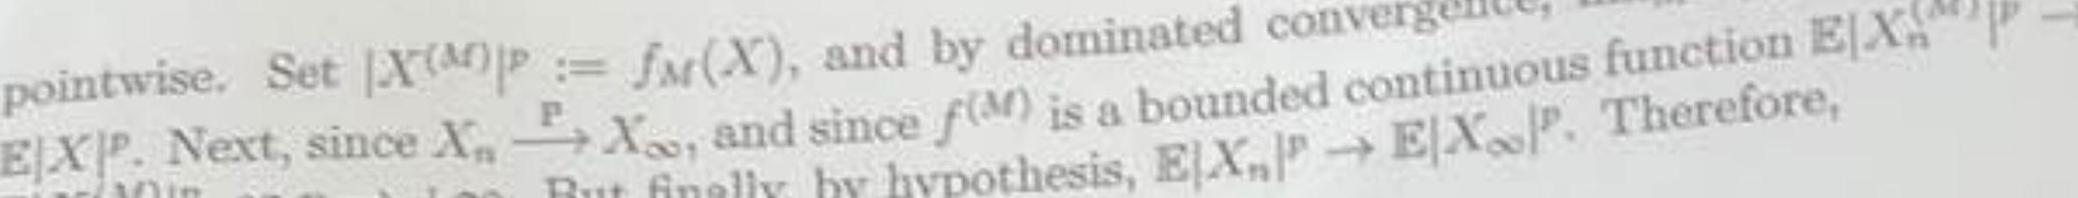
\includegraphics[max width=\textwidth]{2024_11_17_7987aa6f5f165d92ff66g-10} $\mathbb{E}\left|X^{(M)}\right|^{P}$, as $n \rightarrow+\infty$. But finally, by hypothesis, $\mathbb{E}\left|X_{n}\right|^{p} \rightarrow \mathbb{E}\left|X_{\infty}\right|^{\text {P }}$. Therefore,

$$
\begin{aligned}
\mathbb{E}\left|X_{n}\right|{ }^{P} 1_{\mid X n} \mid P \geq M & \leq \mathbb{E}\left|X_{n}\right|^{P}-\mathbb{E} f^{M}\left(\left|X_{n}\right|\right) \\
& \leq \mathbb{E}\left|X_{n}\right|^{p}-\mathbb{E}|X|^{P}+\mathbb{E}|X|^{p}-\mathbb{E}\left|X^{(M) p}+\mathbb{E}\right| X^{(M) \mid P}-\mathbb{E}\left|X_{n}^{(M)}\right|^{p} \\
& \leq \frac{\epsilon}{3}+\frac{\epsilon}{3}+\frac{\epsilon}{3}=\epsilon
\end{aligned}
$$

Here is another slightly different proof of (iii) $\Rightarrow$ (i) which will rely on Lemma 3.14 . let $n(m)$ be a subsequence of integers. Since $X_{n(m)} \xrightarrow{p} X_{\infty}$, there exists a further subsequence $n(m(k))$ such that $X_{n(m(k))} \xrightarrow{a \rightarrow} X_{\infty}$. Then proceeding as above, replacing $n$ by $n(m(k))$ and appealing to the usual Fatou's lemma, gives $\lim \sup _{n(m(k)) \rightarrow+\infty} \mathrm{E}\left|X_{n(m(k))}-X_{\infty}\right|^{p}=0$. Since $L^{p}$ is a metric space, Lemma 3.14 allows to conclude.

The previous theorem asserts that $X_{n} \xrightarrow{L_{p}} X_{\infty}$ if and only if $X_{n} \xrightarrow{p} X_{\infty}$ and $\mathbb{E}\left|X_{n}\right|^{p} \rightarrow$ $\mathbb{E}\left|X_{\infty}\right|^{p}$, if and only if $X_{n} \xrightarrow{p} X_{\infty}$ and $\left(\left|X_{n}\right|^{p}\right)$ is uniformly integrable.

Now that we have studied in detail the various modes of convergence, we will use the tools to prove, at first, some laws of large numbers. These laws are actually theorems asserting that "averages" converge to "probabilities". We begin with a result published in 1859 due to Bienaymé, some one hundred and fifty years after J. Bernoulli proved the result for what is today known as the weak law of large numbers for Bernoulli random variables.\\
Theorem 3.22. Let $X_{1}, X_{2}, \ldots, X_{n}, \ldots$ be iid random variables with $\mathbb{E} X_{1}^{2}<+\infty$. Then

$$
\frac{S_{n}}{n}=\frac{X_{1}+\cdots+X_{n}}{n} \rightarrow \mathbb{E} X_{1},
$$

where the convergence holds in mean square and so in probability.\\
Proof. Let $\epsilon>0$. Then, by the Bienaymé-Chebyshev-Markov inequality,

$$
\begin{aligned}
\mathbb{P}\left(\left|\frac{S_{n}}{n}-\mathbb{E} X_{1}\right| \geq \epsilon\right) & \leq \frac{1}{\epsilon^{2}} \mathbb{E}\left(\frac{S_{n}}{n}-\mathbb{E} X_{1}\right)^{2} \\
& =\frac{1}{n^{2} \varepsilon^{2}} \mathbb{E}\left(S_{n}-\mathbb{E} S_{n}\right)^{2} \\
& =\frac{\operatorname{Var} S_{n}}{n^{2} \epsilon^{2}} \\
& =\frac{\operatorname{Var} X_{1}}{n \epsilon^{2}} .
\end{aligned}
$$

Clearly, $\lim _{n \rightarrow+\infty} \operatorname{Var} X_{1} / n \epsilon^{2}=0$.\\
Above, we not only obtained convergence in probability, but also convergence in $L^{2}$. In fact, as given, the proof does not require the iid assumption but merely for the $X_{1}, X_{2}, \ldots, X_{n}, \ldots$ to be uncorrelated, e.g., pairwise independent, with a uniformly bounded variance.

Next, the finite second moment assumption is removed. This result known as Khintchine weak law of large numbers was published in 1929.

Theorem 3.23. Let $X_{1}, X_{2}, \ldots, X_{n}, \ldots$ be iid random variables with $\mathbb{E}\left|X_{1}\right|<+\infty$. Then,\\
for all $\epsilon>0$,

$$
\lim _{n \rightarrow+\infty} \mathbb{P}\left(\left|\frac{S_{n}}{n}-\mathbb{E} X_{1}\right| \geq \epsilon\right)=0
$$

Proof. The proof techniques involve a truncation argument which is standard in such results and, in fact, convergence holds in $L^{1}$. Indeed, let $M>0$ and let $\widetilde{X}_{k}=X_{k} \mathbf{1}_{\left|X_{k}\right| \leq M}$ and let $\widetilde{S}_{n}=\sum_{k=1}^{n} \widetilde{X}_{k}$. Then, the $\widetilde{X}_{k}$ are bounded iid random variables and so from the previous weak law, $\lim _{n \rightarrow+\infty} \mathbb{E}\left|\tilde{S}_{n} / n-\mathbb{E} \tilde{X}_{1}\right|=0$. Now,

$$
\mathbb{E}\left|\frac{S_{n}}{n}-\mathbb{E} X_{1}\right| \leq \mathbb{E}\left|\frac{S_{n}}{n}-\frac{\widetilde{S}_{n}}{n}\right|+\mathbb{E}\left|\frac{\widetilde{S}_{n}}{n}-\mathbb{E} \widetilde{X}_{1}\right|+\left|\mathbb{E} \tilde{X}_{1}-\mathbb{E} X_{1}\right|
$$

But,

$$
\mathbb{E}\left|S_{n}-\widetilde{S}_{n}\right| \leq \sum_{k=1}^{n} \mathbb{E}\left|X_{k} \mathbf{1}_{\left|X_{k}\right|>M}\right|=n \mathbb{E} \mid X_{1} \mathbf{1}_{\left|X_{1}\right|>M \mid} .
$$

It thus follows that

$$
\limsup _{n \rightarrow+\infty} \mathbb{E}\left|\frac{S_{n}}{n}-\mathbb{E} X_{1}\right| \leq 2 \mathbb{E}\left|X_{1} \mathbf{1}_{\left|X_{1}\right|>M}\right|
$$

Since $\mathbb{E}\left|X_{1}\right|<+\infty$, letting $M \rightarrow+\infty$, finishes the proof.\\
As a well known application of the weak law of large numbers, we give Bernstein's proof of Weierstrass' approximation theorem.\\
Theorem 3.24. Let $f:[a, b] \longrightarrow \mathbb{R}$ be continuous, then $f$ is the uniform limit of polynomials.

Let us now pass to strong convergence results where convergence in probability will be replaced by the almost sure one (ultimately proving it under (pairwise) independence and identical distribution. We start with an easy strong law.\\
Proposition 3.25. Let $p>0$, and let $X_{1}, X_{2}, \ldots, X_{n}, \ldots$ be a sequence of random variables such that $\mathbb{E}\left|X_{k}\right|^{p}<+\infty$. If $\sum_{n=1}^{\infty} \mathbb{E}\left|\frac{S_{n}}{n}\right|^{p,}<+\infty$, then $\frac{S_{n}}{n} \rightarrow 0$, with probability one.\\
Proof. A first proof consists in using the Fubini-Tonelli theorem: since $\mathbb{E} \sum_{n=1}^{\infty}\left|S_{n}\right|^{p} / n^{p}<$ $+\infty$, it follows that $\sum_{n=1}^{\infty}\left|S_{n}\right|^{p} / n^{p}<+\infty$ with probability one, from which one deduces that almost surely $\lim _{n \rightarrow+\infty}\left|S_{n}\right|^{p} / n^{p}=0$. For a second proof, let $\epsilon>0$ then note that

$$
\sum_{n=1}^{\infty} \mathbb{P}\left(\left|\frac{S_{n}}{n}\right| \geq \epsilon\right) \leq \frac{1}{\epsilon^{p}} \sum_{n=1}^{\infty} \mathbb{E}\left|\frac{S_{n}}{n}\right|^{p}<+\infty
$$

and apply Proposition 3.3, i.e., by the Borel-Cantelli lemma the probability of the event $D(\epsilon)=\left\{\left|S_{n} / n\right| \geq \epsilon\right.$ i.o. $\}$ is zero. Since $D$, the set of divergence of $S_{n} / n$ is such that $D \subset U_{\epsilon>0} D(\epsilon)=\cup_{n=1}^{+\infty} D(1 / n)$.

The previous result is rather simple but already shows:\\

\includegraphics[max width=\textwidth, center]{2024_11_17_7987aa6f5f165d92ff66g-12}

Corollary 3.26. Let $X_{1}, X_{2}, \ldots, X_{n}, \ldots$ be iid random variables with $\mathbb{E} X_{1}^{4}<+\infty$. Then,\\
with probability one,

$$
\lim _{n \rightarrow+\infty} \frac{S_{n}}{n}=\mathbb{E} X_{1} .
$$

Proof. Without loss of generality let $\mathbb{E} X_{1}=0$. Then $\mathbb{E}\left(S_{n}-\mathbb{E} S_{n}\right)^{4}=\sum_{i=j} \sum_{k \ell} \mathbb{E} X_{i} X_{j} X_{k} X_{\ell}$. Now by independence if four indices $i, j, k, \ell$ are distincts then $\mathbb{E} X_{i} X_{j} X_{k} X_{\ell}=0$. If four indices are the same then $\mathbb{E} X_{i}^{4}=\mathbb{E} X_{1}^{4}$ and there are $n$ terms of this type. If three indices but not four are the same then again, by independence, $\mathbb{E} X_{i} X_{j}^{3}=0, i \neq j$. So we are left with the terms of the form $\mathbb{E} X_{i}^{2} X_{j}^{2}=\mathbb{E} X_{i}^{2} \mathbb{E} X_{j}^{2}, i \neq j$. There are $\binom{4}{2} n(n-1)$ such terms and each is equal to $\left(\mathbb{E} X_{1}^{2}\right)^{2}$. Now,

$$
\mathbb{E}\left(\frac{S_{n}^{4}}{n^{4}}\right)=\frac{n}{n^{4}} \mathbb{E} X_{1}^{4}+\frac{3 n(n-1)\left(\mathbb{E} X_{1}^{2}\right)^{2}}{n^{4}}
$$

and thus, $\sum_{n=1}^{\infty} \mathbb{E}\left(S_{n}^{4} / n^{4}\right)<+\infty$.\\
We now wish to pass, in the previous result, from a finite fourth moment assumption to a finite second moment assumption.

Theorem 3.27. Let $X_{1}, X_{2}, \ldots, X_{n}, \ldots$ be iid random variables with $\mathbb{E} X_{1}^{2}<+\infty$. Then, with probability one,

$$
\lim _{n \rightarrow+\infty} \frac{S_{n}}{n}=\mathbb{E} X_{1}
$$

Proof. The main idea of the proof is to show that a.s. convergence holds along a dense enough subsequence of integers from which the result will follow. Again, without loss of generality, assume that $\mathbb{E} X_{1}=0$. Then, along the subsequence $n_{k}=k^{2}$, a.s convergence holds true as $\sum_{k=1}^{+\infty} \mathbb{E}\left(S_{n_{k}} / n_{k}\right)^{2}=\sum_{k=1}^{+\infty} \mathbb{E}\left(S_{k^{2}} / k^{2}\right)^{2}=\mathbb{E} X_{1}^{2} \sum_{k=1}^{+\infty} 1 / k^{2}<+\infty$. In other words, for any $\omega \in \widetilde{\Omega}$, with $\mathbb{P}(\widetilde{\Omega})=1, \lim _{k \rightarrow+\infty} S_{k}^{2}(\omega) / k^{2}=0$. Now, for any $k$, let $n=n(k)$ be such that $n_{k}=k^{2} \leq n=n(k)<n_{k+1}=(k+1)^{2}$. Then

$$
\sum_{k=1}^{+\infty} \mathbb{E}\left(\frac{S_{n(k)}}{n(k)}-\frac{S_{k^{2}}}{k^{2}}\right)^{2} \leq 2 \sum_{k=1}^{+\infty}\left(\frac{\mathbb{E} S_{n(k)}^{2}}{n(k)^{2}}+\frac{\mathbb{E} S_{k^{2}}^{2}}{k^{4}}\right) \leq 2 \mathbb{E} X_{1}^{2} \sum_{k=1}^{+\infty}\left(\frac{2 k+1}{k^{4}}+\frac{1}{k^{2}}\right)<+\infty
$$

We therefore proved that for a single $n$ comprised between $k^{2}$ and $(k+1)^{2}$, a.s. convergence holds when $k \rightarrow+\infty$, as we showed that with probability one, $\lim _{k \rightarrow+\infty}\left(S_{n(k)} / n(k)-S_{k^{2}} / k^{2}\right)=$ 0 . However, the result for a single $n=n(k)$ will not be enough and one needs to control the variation for all the variables indexed by the set of $n$ 's between $k^{2}$ and $(k+1)^{2}$. To do so, let

$$
R_{k}:=\sum_{n=k^{2}}^{(k+1)^{2}-1} \mathbb{E}\left(\frac{S_{n}}{n}-\frac{S_{k^{2}}}{k^{2}}\right)^{2}=\sum_{n=k^{2}}^{(k+1)^{2}-1} \mathbb{E}\left(\frac{\sum_{j=1}^{n} X_{j}}{n}-\frac{\sum_{j=1}^{k^{2}} X_{j}}{k^{2}}\right)^{2}
$$

Then,

$$
\begin{aligned}
R_{k} & \leq \mathbb{E} X_{1}^{2} \sum_{n=k^{2}}^{(k+1)^{2}-1}\left(\sum_{j=1}^{k^{2}}\left(\frac{1}{n}-\frac{1}{k^{2}}\right)^{2}+\sum_{j=k^{2}+1}^{n} \frac{1}{n^{2}}\right) \\
& \leq \mathbb{E} X_{1}^{2} \sum_{n=k^{2}}^{(k+1)^{2}-1}\left(\sum_{j=1}^{k^{2}} \frac{\left(k^{2}-n\right)^{2}}{n^{2} k^{4}}+\frac{n-k^{2}}{n^{2}}\right) \\
& \leq \mathbb{E} X_{1}^{2} \sum_{n=k^{2}}^{(k+1)^{2}-1}\left(\frac{\left(k^{2}-n\right)^{2}}{n^{2} k^{4}} k^{2}+\frac{n-k^{2}}{n^{2}}\right) \\
& \leq \mathbb{E} X_{1}^{2}\left(\frac{6 k^{3}}{k^{6}}+\frac{2 k(2 k+1)}{k^{4}}\right) .
\end{aligned}
$$

Therefore, $\sum_{k=1}^{+\infty} R_{k}<+\infty$ and so, with probability one, $\lim _{k \rightarrow+\infty} R_{k}=0$ and thus, with probability one, $\lim _{n \rightarrow+\infty} S_{n} / n=\lim _{k \rightarrow+\infty} S_{k^{2}} / k^{2}=\mathbb{E} X_{1}$.

Another way to prove the above result is to note that the maximal fluctuations between $S_{n} / n$ and $S_{n_{k}} / n_{k}$ is asymptotically zero. Indeed,

$$
\begin{aligned}
\mathbb{P}\left(\max _{n_{k} \leq n<n_{k+1}}\left|\frac{S_{n}}{n}-\frac{S_{n_{k}}}{n_{k}}\right| \geq \epsilon\right) & =\mathbb{P}\left(\bigcup_{n_{k} \leq n<n_{k+1}}\left\{\left|\frac{S_{n}}{n}-\frac{S_{n_{k}}}{n_{k}}\right| \geq \epsilon\right\}\right) \\
& \leq \sum_{n=n_{k}}^{n_{k+1}-1} \mathbb{P}\left(\left|\frac{S_{n}}{n}-\frac{S_{n_{k}}}{n_{k}}\right| \geq \epsilon\right) \\
& \leq \sum_{n=n_{k}}^{n_{k+1}-1}\left(\mathbb{P}\left(\left|\frac{S_{n}-S_{n_{k}}}{n_{k}}\right| \geq \frac{\epsilon}{2}\right)+\mathbb{P}\left(\frac{\left(n-n_{k}\right)}{n n_{k}}\left|S_{n}\right| \geq \frac{\epsilon}{2}\right)\right) \\
& \leq \sum_{n=n_{k}}^{n_{k+1}-1}\left(\frac{4 \mathbb{E}\left(S_{n}-S_{n_{k}}\right)^{2}}{\epsilon^{2} n_{k}^{2}}+\frac{4\left(n-n_{k}\right)^{2} \mathbb{E} S_{n}^{2}}{\epsilon^{2} n^{2} n_{k}^{2}}\right) \\
& \leq \sum_{n=n_{k}}^{n_{k+1}-1}\left(\frac{4\left(n-n_{k}+1\right) \mathbb{E} X_{1}^{2}}{\epsilon^{2} n_{k}^{4}}+\frac{4\left(n-n_{k}\right)^{2} n \mathbb{E} X_{1}^{2}}{\epsilon^{2} n^{2} n_{k}^{2}}\right) \\
& \leq 2 k \mathbb{E} X_{1}^{2}\left(\frac{4(2 k+1)}{\epsilon^{2} k^{4}}+\frac{4(2 k+1)^{2}}{\epsilon^{2} k^{6}}\right)
\end{aligned}
$$

when $n_{k}=k^{2}$. So, letting $D_{k, \epsilon}=\left\{\max _{n_{k} \leq n<n_{k+1}}\left|\frac{S_{n}}{n}-\frac{S_{n_{k}}}{n_{k}}\right| \geq \epsilon\right\}$, it follows by subadditivity and since for $\epsilon_{1}>\epsilon_{2}, D_{k, \epsilon_{1}} \subset D_{k, \epsilon_{2}}$, that

$$
\mathbb{P}\left(\cup_{\epsilon>0}\left\{D_{k, \epsilon} \text { i.o. }(\mathrm{k})\right\}\right)=\mathbb{P}\left(\cup_{m=1}^{+\infty}\left\{D_{k, 1 / m} \text { i.o. }(\mathrm{k})\right\}\right)=0 \text {. }
$$

Finally, $C_{1}=\left\{\lim _{k \rightarrow+\infty} S_{k^{2}} / k^{2}=\mathbb{E} X_{1}\right\}$, and $C_{2}=\mathbb{P}\left(\cap_{m=1}^{+\infty}\left\{D_{k, 1 / m} \text { for infinitely many k }\right\}^{c}\right)$ both have full probability and since $C_{1} \cap C_{2} \subset\left\{\lim _{n \rightarrow+\infty} S_{n} / n=\mathbb{E} X_{1}\right\}$, the result follows.

In the above proof, pairwise independence is enough to get almost sure convergence and, in fact, more generally, the following holds:\\

\includegraphics[max width=\textwidth, center]{2024_11_17_7987aa6f5f165d92ff66g-14}

Theorem 3.28. Let $X_{1}, X_{2}, \ldots, X_{n}, \ldots$ be uncorrelated random variables such that $\sup _{n} \mathbb{E}\left(X_{n}-\right.$ $\left.\mathbb{E} X_{n}\right)^{2}<+\infty$. Then, with probability one,

$$
\lim _{n \rightarrow+\infty} \frac{S_{n}-\mathbb{E} S_{n}}{n}=0 .
$$

We now wish to pass, in the previous theorem, from a finite second moment assumption to a finite first moment assumption. To do so, we will use a (standard) truncation technique.

Theorem 3.29. Let $X_{1}, X_{2}, \ldots, X_{n}, \ldots$ be iid random variables with $\mathbb{E}\left|X_{1}\right|<+\infty$. Then, with probability one,

$$
\lim _{n \rightarrow+\infty} \frac{S_{n}}{n}=\mathbb{E} X_{1} .
$$

Proof. Let $Y_{n}=X_{n} \mathbf{1}_{\left|X_{n}\right| \leq n}$ be the truncation of $X_{n}$ at level $n$ and let $T_{n}=\sum_{k=1}^{n} Y_{k}$. Then,

$$
\frac{S_{n}}{n}-\mathbb{E} X_{1}=\frac{S_{n}-T_{n}}{n}+\frac{T_{n}-\mathbb{E} T_{n}}{n}+\frac{\mathbb{E} T_{n}}{n}-\mathbb{E} X_{1} .
$$

Then, note that by dominated or monotone convergence, $\mathbb{E} Y_{n}=\mathbb{E} X_{n} \mathbf{1}_{\left|X_{n}\right| \leq n}=\mathbb{E} X_{1} \mathbf{1}_{\left|X_{1}\right| \leq n} \rightarrow$ $\mathbb{E} X_{1}$, as $n \rightarrow+\infty$, and so $\lim _{n \rightarrow+\infty} \mathbb{E} T_{n} / n=\mathbb{E} X_{1}$. Also, $\sum_{n=1}^{+\infty} \mathbb{P}\left(X_{n} \neq Y_{n}\right)=\sum_{n=1}^{+\infty} \mathbb{P}\left(\left|X_{n}\right|>\right.$ $n)=\sum_{n=1}^{+\infty} \mathbb{P}\left(\left|X_{1}\right|>n\right) \leq \mathbb{E}\left|X_{1}\right|<+\infty$. Theorefore, by the Borel-Cantelli lemma, $\left\{X_{n}=Y_{n}\right.$ i.o. $\}$ has full probability (such sequences are said to be equivalent sequences or equivalent sequences for almost sure convergence). In other words for all $\omega \in \widetilde{\Omega}$, with $\mathbb{P}(\widetilde{\Omega})$, there exists $n_{0}=n_{0}(\omega)$ such that for all $n \geq n_{0}, X_{n}(\omega)=Y_{n}(\omega)$, so clearly for such $\omega$, the numerical sequences $\left(X_{n}(\omega)\right)_{n \geq 1}$ and $\left(Y_{n}(\omega)\right)_{n \geq 1}$ only differ by finitely many terms, and so $\lim _{n \rightarrow+\infty}\left(S_{n}(\omega)-T_{n}(\omega)\right) / n=0$. We are now left with showing that with probability one, $\lim _{n \rightarrow+\infty}\left(T_{n}-\mathbb{E} T_{n}\right) / n=0$. Since $X_{1}=X_{1}^{+}-X_{1}^{-}$and since both $X_{1}^{+}$and $X_{1}^{-}$have finite first moment and are independent of each other, assume without loss of generality that $X_{1}$ is non-negative. Next, let $\alpha>1$ and let $n_{k}=\left[\alpha^{k}\right]$.

$$
\begin{aligned}
\sum_{k=1}^{+\infty} \mathbb{P}\left(\left|\frac{T_{n_{k}}}{n_{k}}-\frac{\mathbb{E} T_{n_{k}}}{n_{k}}\right| \geq \epsilon\right) & \leq \sum_{k=1}^{+\infty} \frac{1}{\epsilon^{2} n_{k}^{2}} \sum_{m=1}^{n_{k}} \operatorname{Var} Y_{m} \\
& \leq \frac{1}{\epsilon^{2}} \sum_{m=1}^{+\infty} \operatorname{Var} Y_{m} \sum_{n_{k}=m}^{+\infty} \frac{1}{n_{k}^{2}} \\
& \leq \frac{1}{\epsilon^{2}} \sum_{m=1}^{+\infty} \operatorname{Var} Y_{m} \frac{1}{m^{2}} \sum_{k=0}^{+\infty} \frac{1}{\alpha^{2 k}} \\
& =\frac{1}{\epsilon^{2}\left(1-\alpha^{-2}\right)} \sum_{m=1}^{+\infty} \frac{\operatorname{Var} Y_{m}}{m^{2}}
\end{aligned}
$$

To continue, let us show that this last expression is finite. Indeed,

$$
\begin{aligned}
\sum_{m=1}^{+\infty} \frac{\operatorname{Var} Y_{m}}{m^{2}} & \leq \sum_{m=1}^{+\infty} \frac{\mathbb{E} X_{m}^{2} 1_{X_{m} \leq m}}{m^{2}} \\
& =\sum_{m=1}^{+\infty} \frac{1}{m^{2}} \int_{0}^{+\infty} \mathbb{P}\left(X_{m}^{2} \mathbf{1}_{X_{m} \leq m} \geq t\right) d t \\
& =\sum_{m=1}^{+\infty} \frac{1}{m^{2}} \int_{0}^{+\infty} \mathbb{P}\left(m \geq X_{m} \geq \sqrt{t}\right) d t \\
& =\sum_{m=1}^{+\infty} \frac{1}{m^{2}} \int_{0}^{+\infty} \mathbb{P}\left(m \geq X_{1} \geq \sqrt{t}\right) d t \\
& =\sum_{m=1}^{+\infty} \frac{1}{m^{2}} \int_{0}^{m^{2}} \mathbb{P}\left(m \geq X_{1} \geq \sqrt{t}\right) d t \\
& \leq \sum_{m=1}^{+\infty} \frac{1}{m^{2}} \int_{0}^{m^{2}} \mathbb{P}\left(X_{1} \geq \sqrt{t}\right) d t \\
& =\int_{0}^{+\infty} \sum_{m \geq \sqrt{t}} \frac{1}{m^{2}} \mathbb{P}\left(X_{1} \geq \sqrt{t}\right) d t \\
& \leq \int_{0}^{+\infty} \frac{2}{\sqrt{t}} \mathbb{P}\left(X_{1} \geq \sqrt{t}\right) d t=4 \mathbb{E} X_{1}<+\infty
\end{aligned}
$$

Therefore, with probability one, $\lim _{k \rightarrow+\infty} T_{n_{k}} / n_{k}=\mathbb{E} X_{1}$. Now since $X_{1} \geq 0$,

$$
\frac{T_{n_{k}}}{n_{k+1}} \leq \frac{T_{n}}{n} \leq \frac{T_{n_{k+1}}}{n_{k}}
$$

and so, with probability one,

$$
\frac{\mathbb{E} X_{1}}{\alpha} \leq \liminf _{n \rightarrow \infty} \frac{T_{n}}{n} \leq \limsup _{n \rightarrow \infty} \frac{T_{n}}{n} \leq \alpha \mathbb{E} X_{1}
$$

Taking $\alpha=1+1 / r$, finally shows that, with probability one, $\lim _{n \rightarrow+\infty} T_{n} / n=\mathbb{E} X_{1}$.\\
The proof of the SLLN shows that the iid assumption can be replaced by pairwise independent with identical distribution. However, $\mathbb{E}\left|X_{1}\right|<+\infty$ cannot be removed as show next.

Corollary 3.30. Let $X_{1}, X_{2}, \ldots, X_{n}, \ldots$ be non-negative iid random variables variables such that $\mathbb{E} X_{1}=+\infty$. Then, with probability one, $\lim _{n \rightarrow+\infty} S_{n} / n=+\infty$.\\
Proof. Let $M>0$. Then, $X_{n} \geq Y_{n}:=X_{n} 1_{\left\{0 \leq X_{n} \leq M\right\}}+M 1_{\left\{X_{n}>M\right\}}=\min \left(X_{n}, M\right)$. Then, the $Y_{n}$ 's are non-negative iid random variables with $\mathbb{E} Y_{1}<+\infty$. Therefore by the SLLN, with probability one,

$$
\lim _{n \rightarrow+\infty} \frac{S_{n}}{n} \geq \lim _{n \rightarrow+\infty} \frac{1}{n} \sum_{k=1}^{n} \min \left(X_{k}, M\right)=\mathbb{E} Y_{1}=\mathbb{E} \min \left(X_{1}, M\right) \longrightarrow+\infty
$$

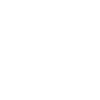
\includegraphics[max width=\textwidth, center]{image-not-found}\\
as $M \rightarrow+\infty$. of iid random variables be such that $\mathbb{P}\left(X_{1}=|n|\right)=c / n^{2} \ln (1+|n|), n \geq 1$, where $c>$\\
0 is a normalizing constant. Then $\left.\mathbb{E}\left|X_{1}\right|=\mid X_{n}\right)_{n}$ $\lim \sup _{n \rightarrow+\infty} S_{n} / n=+\infty$ while $\liminf _{n \rightarrow+\infty} S_{n} / n=+\infty$ and so the SLLN fails and, in fact, and $S_{n} / n$ converges in probability towards $0 "=-\infty$, but $\left(X_{n}\right)_{n \geq 1}$ satisfies the WLLN,\\
$=" \mathbb{E} X_{1}$. providing, in particular, ander is devoted to studying series of independent random variables numbers in case of iid random variables (original to Kolmogorov) of the strong law of large

You hnow that $\sum_{n=1}^{\infty} \frac{1}{n}$ divenge but $\sum_{n=1}^{\infty} \frac{(-1)^{n}}{n}$ can renge. $(-1)^{n}$ can be deen as $-1,1,-1,1, \ldots$\\
Replace $(-1)^{n}$ by $X_{n}$, whe $X_{n}= \begin{cases}-1 & \text { w.p. } \frac{1}{2} \\ +1 & \text { w.p. } \frac{1}{2}\end{cases}$\\
$\sum_{n=1}^{\infty} \frac{x_{n}}{n}$,\\
$C=\left\{w: \sum_{n=1}^{\infty} \frac{X_{n}}{n}(\omega) \angle+\infty\right\}$. Has C postine\\
measure?. Fram Kolmogoov's 0-1 law $\mathbb{P}(C)=0$ a 1.\\
Wart to fird criteria tensung thel. $\sum X_{n}$ caveys.\\
Therem 3.25 led $x_{1}, x_{2}, \ldots, x_{n}, \ldots$ be $\frac{11}{0}$ n.v., if\\
(i) $\sum_{n=1}^{\infty} V_{a n} X_{n} L+\infty$, then $\sum_{n=1}^{\infty}\left(X_{n}-E X_{n}\right)$ converges a - s.\\
(4) If moncouen $\left\|X_{n}^{l}\right\|_{\infty}^{-\mathbb{E} x_{n}} \leqslant c, \forall n \geqslant 1$, the comense is time.

Kolmogaev Maxinal Ine sualtey\_\\
(a) lel $x_{2}, x_{2}, \ldots, x_{n}, \ldots$ be $\Perp_{1 . v}$. wh $\notin X_{e}^{2} c+\infty$. Then, $\forall \varepsilon>0$

$$
\mathbb{P}\left(\max _{1 \leq h \leq n}\left|S_{e r}-\mathbb{A} S_{e r}\right| \geqslant \varepsilon\right) \leqslant \frac{V_{m e} \delta_{n}}{\varepsilon^{2}}
$$

(b) Moreane, if $\left\|X_{n}^{\prime}\right\|_{\infty}^{\pi X_{n}} \leq c, \forall n \geqslant 1$, then

$$
\mathbb{P}\left(\max _{1 \leqslant n \leqslant n}\left|S_{n}-\mathbb{E} S_{\text {en }}\right| \geqslant \varepsilon\right) \geqslant 1-\frac{(c+\varepsilon)^{2}}{\operatorname{Van} S_{n}}
$$

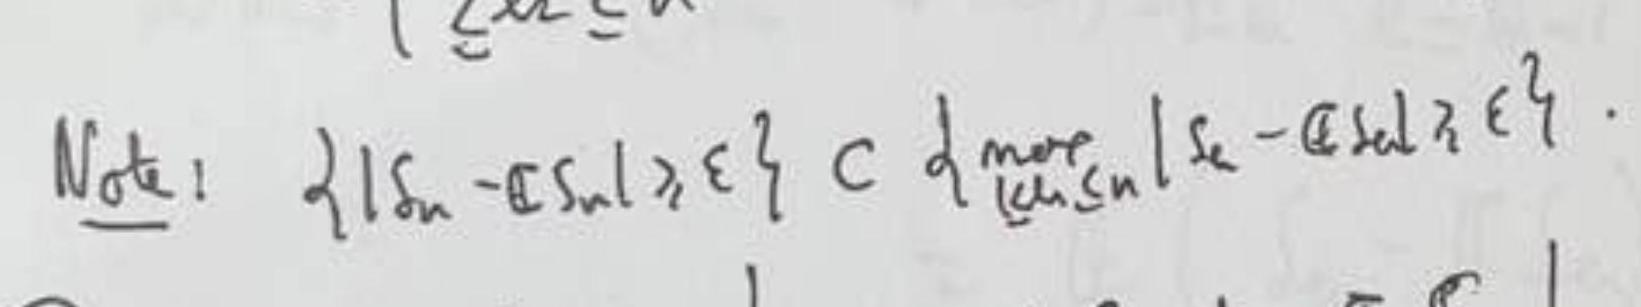
\includegraphics[max width=\textwidth, center]{2024_11_17_7987aa6f5f165d92ff66g-18}\\
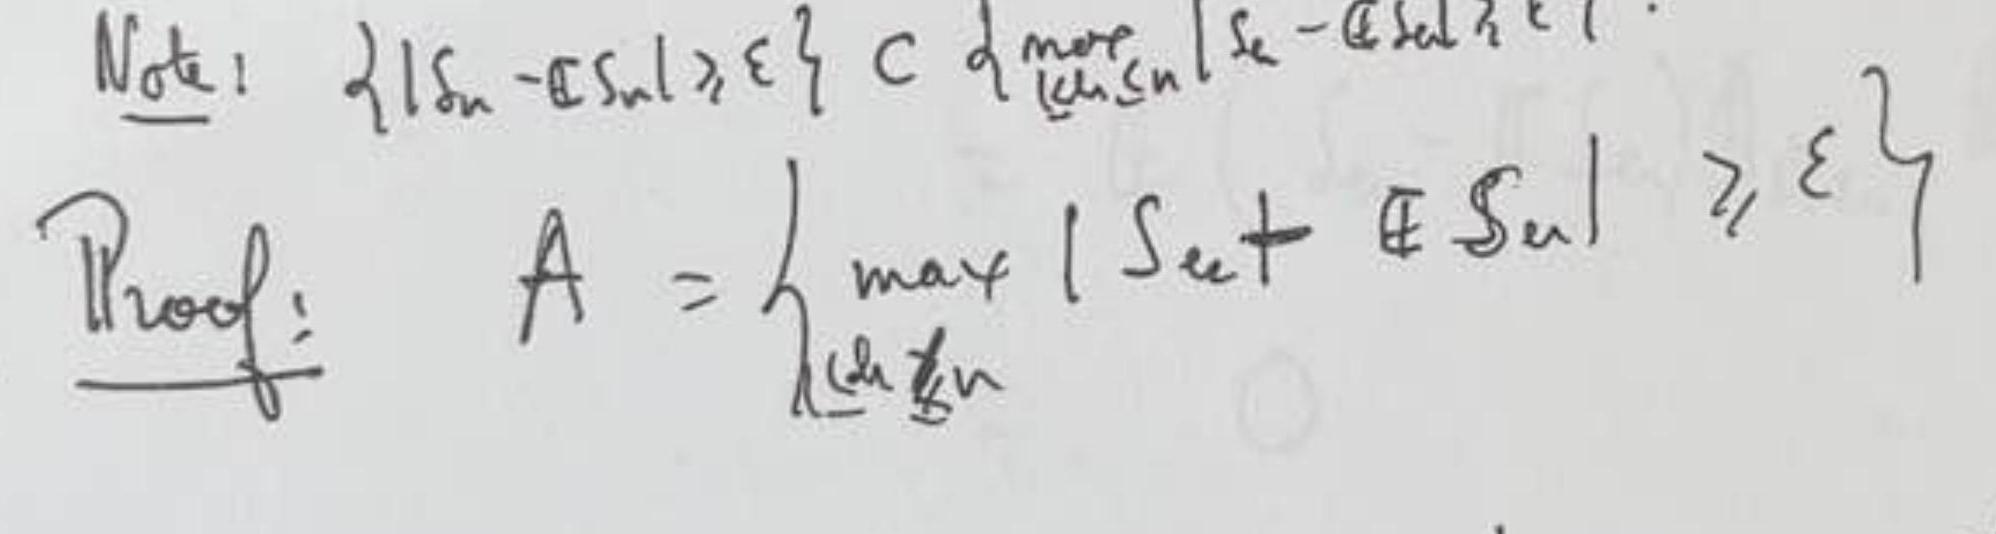
\includegraphics[max width=\textwidth, center]{2024_11_17_7987aa6f5f165d92ff66g-18(1)}

$$
\begin{aligned}
& V_{a r} S_{n}=\mathbb{E}\left(S_{n}-\mathbb{E} S_{n}\right)^{2} \geqslant \mathbb{E}\left(\left(S_{n}-\mathbb{E} S_{n}\right)^{2} \underline{I}_{A}\right) \\
& =\sum_{n=1}^{n} \mathbb{E}\left(S_{n}-\mathbb{E} S_{n}\right)^{2} \mathbb{1}_{A a}
\end{aligned}
$$

$$
\begin{aligned}
& \left.\mathbb{E}\left(S_{n}-\mathbb{E} S_{n}\right)^{2} \mathbb{1}_{A_{n}}=\mathbb{E}\left(\left[S_{a}-\mathbb{Q} S_{n e n}\right)+\sum_{e=k+1}^{n}\left(\alpha_{e}-\mathbb{E} X_{e}\right)\right]^{2} \mathbb{A}_{A_{n}}\right)
\end{aligned}
$$

$$
\begin{aligned}
& \left.+\left(\sum_{l=n+1}^{n}\left(X_{l}-\Phi X_{l}\right)\right)^{2} 1_{A_{n}}\right)
\end{aligned}
$$

Now $\mathbb{E}\left(S_{l}-\mathbb{E} S_{e}\right) \mathbb{1}_{A a} \sum_{l=h+1}^{n}\left(X_{l}-\mathbb{E} X_{l}\right)$

$$
\begin{aligned}
& =\mathbb{E}\left(\delta_{h}-\mathbb{E} S_{e}\right) \mathbb{I}_{A_{h}} \mathbb{E} \sum_{l=k+1}^{n}\left(X_{l}-\mathbb{E} X_{l}\right) \\
& =0
\end{aligned}
$$

Hence

$$
\begin{aligned}
& w^{a} \\
& \mathbb{E}\left(S_{n}-\mathbb{E} S_{n}\right)^{2} \mathbb{1}_{A a} \geqslant \mathbb{E}\left(\left(S_{a}-\mathbb{E} S_{e n}\right)^{2} \mathbb{1}_{A+a}\right) \\
& \geqslant \varepsilon^{2} \mathbb{P}\left(A_{n}\right) .
\end{aligned}
$$

Thees, $\frac{V a_{n} S_{n}}{\varepsilon^{2}} \geqslant \sum_{e=1}^{n} \mathbb{P}\left(A_{n}\right)=\mathbb{P}(A)$.

Fa be neverse ine qualty

$$
\begin{aligned}
& \mathbb{E}\left(S_{n}-\mathbb{E} S_{n}\right)^{2} \mathbb{1}_{A}=\operatorname{Var} S_{n}-\mathbb{E}\left(S_{n}-\mathbb{E} S_{n}\right)^{2} \mathbb{1}_{A^{c}} \\
& \geqslant \operatorname{Var} S_{n}-\varepsilon^{2} \mathbb{P}\left(A^{c}\right) \\
&=\operatorname{Var} S_{n}-\varepsilon^{2}+\varepsilon^{2} \mathbb{P}(A) \quad(*) \\
& N_{\text {aw }} \text { on } A_{e n},\left|S_{e r-1}-\mathbb{E} S_{a-1}\right| \leq \varepsilon
\end{aligned}
$$

Now on Aer, $\left|S_{e r-1}-\mathbb{E} S_{e-1}\right| \leq \mathbb{E}$

$$
\text { and } \begin{aligned}
&\left|S_{e}-\Phi S_{u}\right| \leq\left|S_{u-1}-\mathbb{E} S_{u-1}\right|+ \\
&\left|X_{e}-\mathbb{E} x_{e n}\right| \\
& \leq \varepsilon+C
\end{aligned}
$$

Hence

$$
\begin{aligned}
& \operatorname{Var} S_{n} \mathbb{1}_{A}=A_{A} \in\left(S_{n}-\mathbb{A} S_{n}\right)^{2} \mathbb{1}_{A_{n}} \\
& =\sum_{n=1}^{n} \mathbb{E}\left(S_{n}-\mathbb{E} S_{n}\right)^{2} \mathbb{U}_{A e r}
\end{aligned}
$$

$$
\begin{aligned}
& \leq(\varepsilon+c)^{2} \sum_{\mu=1} \mathbb{P}\left(A_{n}\right)+\sum_{\mu=1}^{n} \mathbb{P}\left(A_{\mu}\right) \sum_{l=h+1} \mathbb{E}\left(X_{l}-\mathbb{E} X_{l}\right)^{2} \\
& =\mathbb{P}(A)\left((\varepsilon+c)^{2}+\sum_{l=h+1}^{n} V_{a r} X_{l}\right) \\
& \leq \mathbb{P}(A)\left((\varepsilon+c)^{2}+V_{a r} S_{n}\right) \quad(b)
\end{aligned}
$$

Naw frem (8) and (*k) we get

$$
\begin{aligned}
& V_{a r} S_{n}-\varepsilon^{2}+\varepsilon^{2} \mathbb{P}(A) \leq \operatorname{Var}_{n} \mathbb{1}_{A} \leq \mathbb{P}(A)\left((\varepsilon+c)^{2}+V_{a r} S_{n}\right) \\
& \operatorname{Van} \delta_{n}-\varepsilon^{2} \leq \mathbb{P}(A)\left((\varepsilon+C)^{2}-\varepsilon^{2}+V_{a r} S_{n}\right)
\end{aligned}
$$

Hence

$$
\begin{aligned}
\mathbb{P}(A) \geqslant \frac{V_{a r} S_{n}-\varepsilon^{2}}{(\varepsilon+c)^{2}-\varepsilon^{2}+V_{a r} S_{n}} & =1-\frac{(\varepsilon+c)^{2}}{(\varepsilon+c)^{2}+V_{a} S_{n}-\varepsilon^{2}} \\
& \geqslant 1-\frac{(\varepsilon+c)^{2}}{V_{a r} S_{n}}
\end{aligned}
$$

Proof of the Theorem 3.25 of partial\\
(6) The cons. convergence of the sequence is equiv cleat to.

$$
\lim _{n \rightarrow+\infty} \mathbb{P}\left(\sup _{k \geqslant 1}\left|S_{n+h}^{-\mathbb{D S}+\ldots+n} S_{n}^{\prime}\right| \geqslant \varepsilon\right)=0
$$

\begin{center}
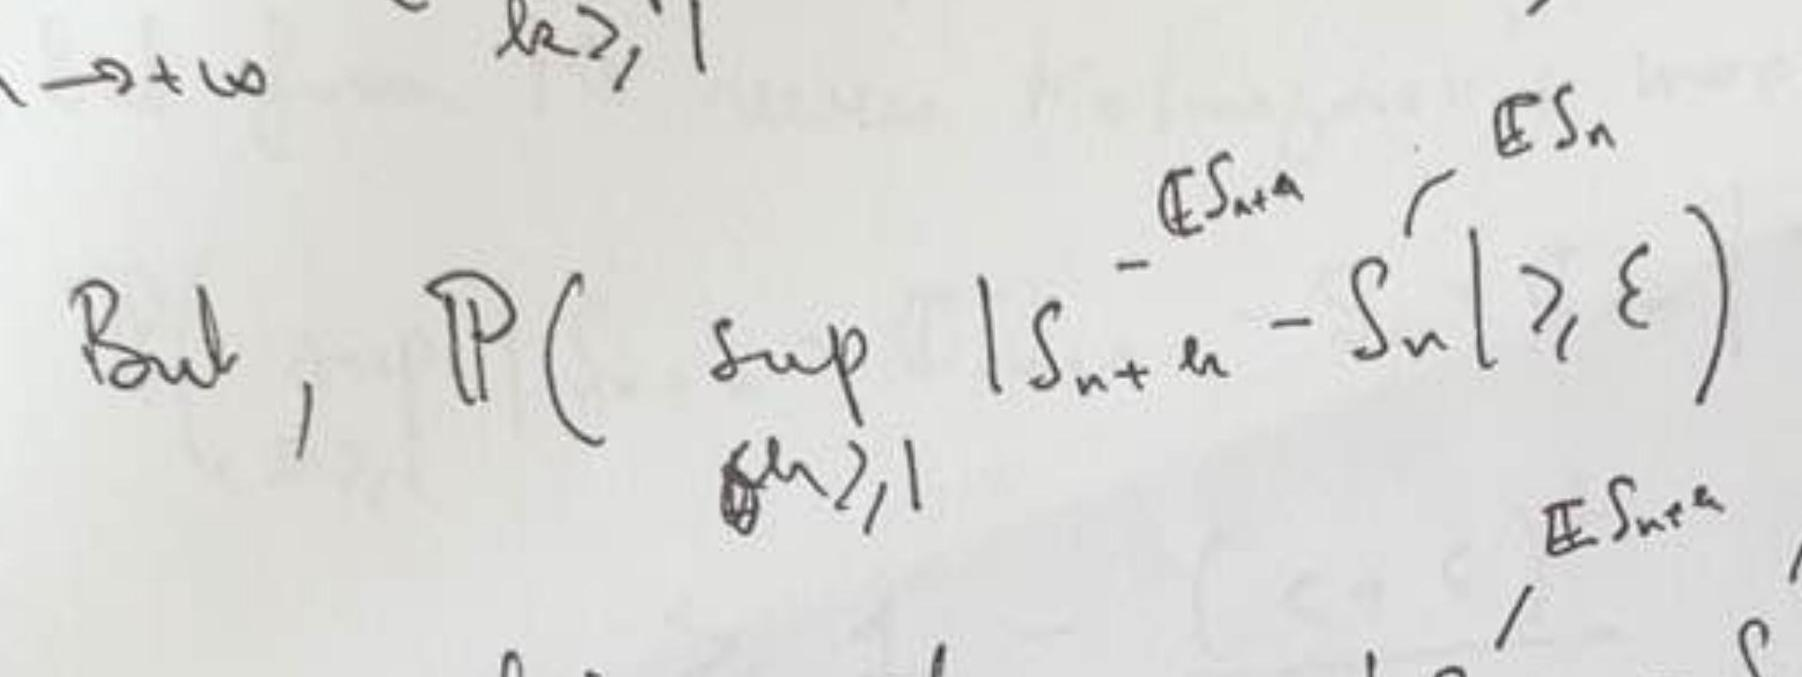
\includegraphics[max width=\textwidth]{2024_11_17_7987aa6f5f165d92ff66g-22}
\end{center}

$$
\begin{aligned}
& =\lim _{N \rightarrow+\infty} \mathbb{P}\left(\max _{1 \leq h \leq N}\left|S_{n+n}^{\prime} \operatorname{ISn}_{n+N}-S_{n}^{\prime}\right| \geqslant \varepsilon\right) \\
& \leq \lim _{N \rightarrow+\infty} \frac{\sum_{\mu=n}^{n+N} V_{a r} X_{\mu}}{\varepsilon^{2}}=\frac{\sum_{\mu=n}^{\infty} V_{a} X_{e}}{\varepsilon^{2}} \text {. }
\end{aligned}
$$

Therefore, if $\sum_{s=1}^{\infty} V_{a r} X_{s}<+\infty$, then, $\sum_{n=1}^{\infty}\left(X_{n}-\mathbb{E} X_{n}\right)$ converges a.s.\\
then for $n$ lange enough,

$$
\mathbb{P}\left(\sup _{n \geqslant 1}\left|S_{n+k}-E_{n+a}-S_{n}+\mathbb{E} S_{n}\right| \geqslant \varepsilon\right)<\frac{1}{2} .
$$

But from the reues $K_{0} /$ magaov's moximal inegwalt,

$$
\begin{gathered}
\mathbb{P}\left(\sup _{n \geqslant 1}\left|S_{n+h}-\mathbb{C} S_{n+h}-S_{n}+\mathbb{E} S_{n}\right| \geqslant \varepsilon\right) \\
\geqslant 1-\frac{(c+\varepsilon)^{2}}{\sum_{e=n+1}^{\infty} \operatorname{Var} X_{e n}}
\end{gathered}
$$

Terefore, if $\sum_{\mu=1}^{\infty} V_{a n} X_{n}=+\infty$, we geel.

$$
\mathbb{P}\left(\sup _{n \geqslant 1}\left|S_{n+e}-\mathbb{E} S_{n+n}-S_{n}+\mathbb{E} S_{n}\right| \geqslant \varepsilon\right)=1 .
$$

Note: Cel $x_{1}, x_{2}, \ldots, x_{n}, \ldots$ be iid N.V with $\mathbb{P}\left(X_{2}=1\right)=\mathbb{P}\left(X_{1}=-1\right)=\frac{1}{2}$.\\
$\sum_{i=1}^{\infty} x \quad\left|x_{1}\right| \leqslant 1$. Therefore.\\
$\sum_{n=1} a_{n} X_{n}$ comerges $a_{0} s$. iff $\sum_{n=1}^{\infty} V_{a n} a_{n} X_{n} c+\infty$\\
iff $\sum_{n=1}^{\infty} a_{n}^{2} c+\infty$.\\
Deem 3.27 . (Two series theorem) let $x_{1}, x_{2}, \ldots, x_{n}, \cdots$ be II riv. The ar, such that $\sum_{n=1}^{\infty} \oplus X_{n}<+\infty$ ad $\sum_{n=1}^{\infty} \operatorname{Van} X_{n}<+\infty$, then $\sum_{n=1}^{\infty} X_{n}$ converges ass. Conversely, if $\left\|X_{n}^{-}\right\|_{\infty}^{C X_{m}^{n}=1} \leq C$, the convergence of the two series is alow necessary for the convergence of $\sum_{n=1}^{\infty} X_{n}$.\\
Proof: If $\sum_{n=1}^{\infty} V_{a r} x_{n} c+\infty$, then $\sum_{n=1}^{\infty}\left(x_{n}-\mathbb{E} x_{n}\right)$ converges al mat surely. But if $\sum_{n=1}^{\infty} \Subset X_{n}$ converges then $\sum_{n=1}^{\infty} X_{n}$ converges ass.\\
, we wor a symuetization trice inde $, \cdots, \mathbb{P})$ conture $\tilde{x}_{1}, \tilde{x}_{2}, \cdots, \tilde{x}_{n}, \cdots$ irdependent $n \cdot v$ s.l $\quad X_{n} \stackrel{d}{=} \tilde{X}_{n}^{\prime}$. Nom, if $\sum X_{n}$ comery. $a_{-1}$, so does $\sum \tilde{X}_{n}$ and thes So doe $\sum\left(x_{n}-\tilde{x}_{n}\right)$. But $\mathbb{E}\left(x_{n}-\tilde{x}_{n}\right)=0$ and $\left\|X_{n}-\tilde{X}_{n}\right\|_{\infty} \leqslant 2 c$. Thearfare by Theorem 3.25, $\sum_{n=1}^{\infty} \operatorname{Var}\left(X_{n}-\tilde{X}_{n}\right)<+\infty$. Bal $\sum_{n=1}^{n} \operatorname{Var}\left(X_{n}-\tilde{X}_{n}\right)=2 \sum_{n=1}^{n} \operatorname{Var} X_{n}$. Rerifare, $\sum_{n=1}^{\infty}\left(X_{n}-\mathbb{E} X_{n}\right)$ conerys a.s and thenefore $\sum_{n=1}^{\infty} \Phi X_{n}$ coneys if $\sum_{n=1}^{\infty} X_{n}$ converges a.s.

Let $X_{1}, X_{1}, \ldots, X_{4}, \ldots$ be a sequence of U n.v. Let $M>0$ and le b fer each $h=1,2,-$\\
$X_{e}^{(M)}=\left\{\begin{array}{ll}X_{\mu} & \text { if }\left|X_{\mu}\right| \leqslant M \\ 0 & \text { if }\left|X_{e 2}\right|>M\end{array}\right.$. If the series, $\sum X_{n}$\\
(a) $\sum \mathbb{E} X_{n}^{(M)}<+\infty$ Then,\\
(b) $\sum \operatorname{Var} X_{n}^{(M)} \angle+\infty$\\
(c) $\sum \mathbb{P}\left(\left|X_{n}\right| \geqslant M\right)<+\infty$\\
far every $M>0$. Car resacly if (a), (b), (c) hold true for same $M>0$, then the series $\sum_{n=1}^{\infty} X_{n}$ converges ass. (and this (2), (0, (c) hold true for even $M>0$ ) if it holds hive for some $M>0$ )\\
Proof: (Sufficiency) By the two series Teem, $\sum_{n=1} X_{n}^{(M)}$ converge alma surely.\\
Now, if $\sum_{n=1}^{n} \mathbb{P}\left(\left|X_{n}\right| \geqslant M\right) \angle+\infty$, then by

Bool-Cantelle, $P\left(\left|X_{n}\right| \geqslant M \quad\right.$ i. o. $)=0$\\
$\left(\sum_{n=1}^{\infty} \mathbb{1}_{\left\{X_{n} \mid \geqslant M\right\}<t \infty}\right)$, Hence $x_{n}=x_{n}^{(0),}$ fa all but fintely mary $n$. Rerefore, $\sum X_{n}$ conveyes a.s.\\
Necuntar. If $\sum X_{n}$ comerges aluat onvely, then $X_{n} \xrightarrow{n \rightarrow+\infty} 0$ a.s. Therefore, for ary $M>0$, anly fintely mary of the events $\left.\mathbb{1}_{\{\mid X, D} \mid M\right\}$ can occum, (1.s.). Therefue $\sum_{n=1}^{\infty} \mathbb{1}_{\left\{\left|X_{n}\right| \geqslant M\right\}} L+\infty$. Bual by the $2^{\text {nd }}$ pert of Beat-Cantelli, $\sum_{n=1}^{\infty} \mathbb{P}\left(\left|X_{n}\right| \geqslant M\right)<-\infty$. Bou, the cervergence of $\sum_{n=1}^{\infty} X_{n}$ unghis the conreyence But, the cernergence of $\sum_{n=1}^{\infty} x_{n}$ ung the two\\
of $\sum_{n=1}^{\infty} X_{n}^{(n)}$ add we cenclude by the orem.

Bythe tersting Bond Centalle: lumar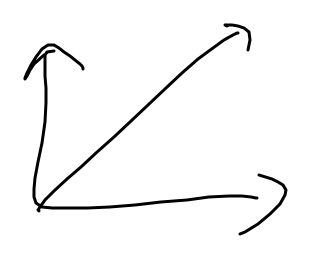
\includegraphics[max width=\textwidth]{62HivP_eDOuGkOPogYMNnG5eK8GI1AO0xqtZc8ncog4_original_fullsize}

Finite elements,


\end{document}